\DiaryEntry{Birthday Problem}{2016-09-16}{Maths}

The birthday problem asks for the probability that 2 (or more) persons in a room with \(r\) people share the same birthday (same day in a year). More exactly, it deals with the probability that \textbf{any} 2 (or more) persons share the same day.

If we allow \(N\) days for a year, we obtain for the probability that no people share a birthday

\[
P = \frac{N(N-1)(N-2) \cdots (N-r+1)}{N^r} = \frac{N!}{(N-r)!N^r}
\]

The first person has \(N\) possibilities, the second one has one less, etc. In total, \(r\) people can have \(N^r\) different birthdays.

The probability for ``birthday collisions'' is then

\[
P = 1 - \frac{N(N-1)(N-2) \cdots (N-r+1)}{N^r} = 1 - \frac{N!}{(N-r)!N^r}
\]

This is ``surprisingly'' high; e.g. \(P_b \approx 1/2\) for \(r=23, N = 365\) and \(P \approx 1\) for about 50 persons. The reason for this is that we are asking for \textbf{any} persons sharing birthday and there is a large number of such pairings; namely \(N(N-1)/2\) (\(N\) for the first choice, \(N-1\) for the second) which increases very quickly.

The Figure below shows the probability as function of \(r\) and \(N=365\).

\begin{figure}[H]
\centering
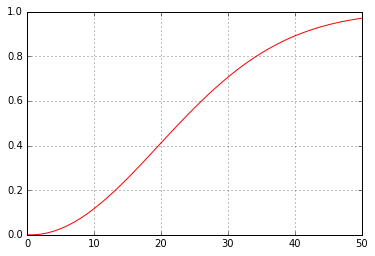
\includegraphics{images/birthday_problem_2.png}
\end{figure}

\subsection{Birthmate Problem}

Here the question is slightly different: We fix the birthday (e.g.~to the observer's birthday) and ask for the probability that one (or more) person has the same birthday.

The probability that no one has the same birthday as we is given by

\[
P = \left( \frac{N-1}{N} \right)^r
\]

Every person has the same chance of \((N-1)/N\) of not sharing birthday and we multiply this over \(r\) persons. The ``collision'' probability is then

\[
P = 1 - \left( \frac{N-1}{N} \right)^r
\]

\subsection{Discussion}

The following Figure shows plots for the birthday problem (red) and the birthmate problem (blue) as function of \(r\) and for \(N=365\).

\begin{figure}[H]
\centering
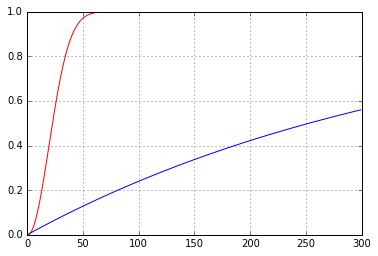
\includegraphics{images/birthday_problem_1.png}
\end{figure}
